\chapter{Algoritmo exacto}
\section{Desarrollo}
Un dibujo incremental valido para el problema, consiste en una permutaci�n de los nodos de cada partci�n que mantenga el orden relativo de los nodos antiguos. Si tenemos $v_i$ nodos inicialmente en la particion i, y se agregan $IV_i$ nodos en cada partici�n, la cantidad posible de soluciones es:
$$IV_1!*\dbinom{IV_1 + v_1}{v_1}*IV_2\dbinom{IV_2 + v_2}{v_2}$$
Esto se debe a que la partici�n 1 tiene $IV_1 + v_1$ nodos, por lo tanto hay esa cantidad de posiciones. De esas tengo que usar $v_1$ para los nodos viejos. Una vez que elegimos las posiciones, el orden entre ellos es fijo, por lo que si elegimos $v_1$ posiciones, solo hay 1 forma de ubicarlos. Pero en las $IV_1$ posiciones que quedan libres podemos poner cualquier permutaci�n de los nodos nuevos. De ahi viene que la cantidad de ordenes v�lidos para la particion 1 sea: 
$$ IV_1!*\dbinom{IV_1 + v_1}{v_1} $$
Para cada una de estas permutaciones, tenemos, haciendo un razonamiento similar a lo visto antes, una cantidad de permutaciones igual a:
$$IV_2!*\dbinom{IV_2 + v_2}{v_2}$$ permutaciones en la segunda partici�n.  

Dada la naturaleza del problema a resolver, lo que planteamos como acercamiento para un algoritmo exacto es utilizar la tecnica de backtracking.

La idea es obtener una soluci�n base de alguna manera, por ejemplo a partir de la heuristica constructiva que desarrollamos mas adelante en la parte \ref{constructivas}, y usar esta soluci�n inicial para poder descartar de las posibles permutaciones de los nodos a las que generan mas cruces, y cada vez que encontramos una permutaci�n que genera menos cruces, utilizamos esa para filtrar al resto. Para armar las soluciones, partimos de los nodos antiguos ya puestos, y vamos llenando la partici�n que tenga menos permutaciones validas (en adelante, le diremos partici�n 1), cuando que llenamos esta, probamos todas las permutaciones de la otra.

De esta manera, el �rbol de backtracking que tenemos es:
\begin{figure}[H]
\centering
\setcounter{subfigure}{0}
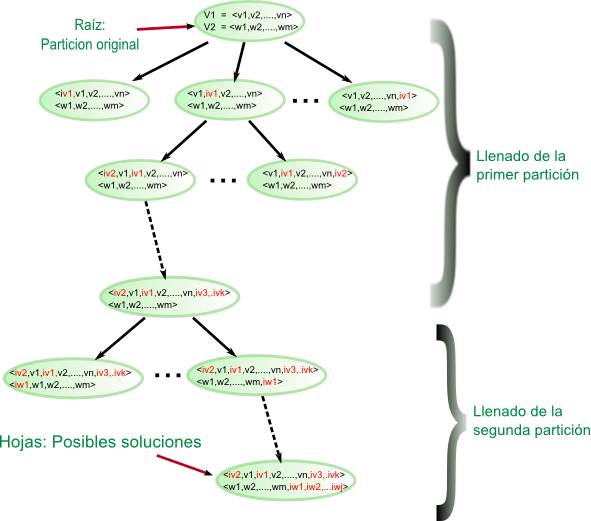
\includegraphics[scale=0.25]{./figuras/exacto/arbolbt.png}
\caption{Arbol de backtracking}
\end{figure}

Nuestro algoritmo lo va recorriendo a la manera de DFS, cortando aquellas ramas que se pueden descartar por tener un n�mero de cruces mas alto que la mejor soluci�n encontrada hasta el momento.

\subsection{Podas}
La poda basica que efectuamos consiste en eliminar aquellas permutaciones que sabemos que no pueden ser soluci�n porque ya tienen mas cruces que otra permutaci�n que armamos. 

Sin embargo, nos gustar�a poder desarrollar alg�n otro tipo de poda, que nos permita mejorar el rendimiento del algoritmo.

Consideremos un dibujo con dos permutaciones $V = <v_1,v_2,...,v_n>$, $W = <w_1,w_2,...,w_k>$, la cantidad de cruces se puede obtener como:

$$Cruces(V,W) = \sum_{i=1}^{k-1}{\sum_{j=i+1}^{k}{crucesEntre( w_i,w_j,V)}}$$

Entonces, una vez que tenemos llena la primer partici�n, podemos obtener una cota inferior para la cantidad de cruces que va a haber en la partici�n 2:

$$Cruces(V,W) \geq \sum_{i=1}^{k-1}{\sum_{j=i+1}^{k}{min(crucesEntre(w_i,w_j,V),crucesEntre(w_j,w_i,V))}}$$

Esto nos dice que dados dos nodos, $w_i$ y $w_j$, sabiendo en que orden estan los nodos de la otra partici�n, hay dos formas de coloarlos y una forma que genera menos cruces (podrian ser las dos formas si son iguales). Entonces en el mejor de los casos, todos los nodos estan ordenados de modo que dado un par cualquiera cumplen que estan en el mejor orden. 

De esta manera, obtenemos una cota que nos permite desarrollar otra poda para aplicar a nuestro algoritmo: Una vez que completamos la primer partici�n, podemos ver antes de agregar un nodo a la segunda partici�n, si los cruces que ya hay entre los nodos puestos, mas este limite inferior para el n�mero de cruces que involucran a los nodos que todavia no pusimos, es mayor que la cantidad de la mejor soluci�n hasta el momento, no vale la pena seguir construyendo esta permutaci�n.

Es de notar que el calculo de esta cota implica un overhead, por eso un factor que deberemos estudiar es si es conveniente aplicarla, ya que en el peor caso, no se poda nunca y el rendimiento es peor que si no usaramos la poda. Entonces algo que debemos observar es si la poda aporta un beneficio o es mas bien un overhead inutil.

\subsection{Tabulado de resultados}
Para ir construyendo las permutaciones, vamos agregando nodos al final, hacemos una llamada recursiva donde agregamos a los otros nodos. Cuando termina una llamada, lo que hacemos es un swap entre el nodo que agregamos y su anterior, y se repite la llamada, asi hasta que el nodo llega al final de la partici�n y hay que sacarlo.

Cada vez que hacemos un swap, calculamos la cantidad de cruces que hay entre dos nodos antes de hacer el swap y despues de hacerlo, para saber cuantos cruces hay en el dibujo que estamos armando.

Si consideramos la primer partici�n, como la armamos primero, resulta que en la partici�n opuesta solo estan los nodos antiguos, cuyo orden es fijo. Por lo cual los cruces entre dos nodos de la primer partici�n, cuando esta todavia no se lleno es siempre la misma. 

Esto quiere decir, que estamos repitiendo calculos, ya que al sacar un nodo y volverlo a poner, calculamos los cruces que genera con los demas, lo cual podriamos haber evitado. Por esta razon, al comenzar el backtracking, calculamos la cantidad de cruces entre dos nodos cualesquiera de la primer partici�n, de modo tal que cuando lo estemos moviendo mediante swaps, no necesitemos calcular nuevamente los cruces que genera con sus compa�eros de partici�n.

Si bien hacer esto, tiene un costo espacial y temporal $O(V_1^2)$, dado el costo que tiene contar los cruces, y la cantidad de veces que es necesario hacerlo, creemos que es una optimizaci�n valida.

De manera similar, cuando se llena la partici�n 1, los cruces entre nodos de otra partici�n son siempre iguales, por esta raz�n cada vez que llenamos a la primer partici�n, calculamos una tabla similar para la segunda. Esta tabla ademas nos es de mucha utilidad para poder calcular la poda antes descripta en un orden mucho menor, ya que todos los valores que necesitamos sumar, ya estan calculados.
 
\section{Pseudocodigo}
\begin{algorithm}[H]
\caption{Resuelve de forma exacta el problema de dibujar grafos incrementales bipartitos}
\begin{algorithmic}[1]
\STATE generar excepci�n de no implementado
\end{algorithmic}
\end{algorithm}

\section{Detalles de implementaci�n}

\section{Calculo de complejidad}

\subsection{Peores casos}

\section{Analisis experimental}

\subsection{Experiencias realizadas}

\subsection{Resultados}

\section{Discusi�n}